\maketitle

\section{实验概括}

我们使用基于 Transformer 架构的大语言模型(Large Language Model,LLM)Llama 3.1 8B\cite{grattafiori2024llama3herdmodels} 在新闻分类领域\textbf{最困难}的数据集 AG News\cite{zhang2015character}上进行全量监督微调(Supervised Fine-Tuning,SFT),在 8 卡 A100 上训练 1 个 epoch,得到的模型在测试集上的准确率为 \textbf{95.43\%},实现了 SOTA(state-of-the-art)级别的性能。
\begin{figure}[htbp]
    \centering
    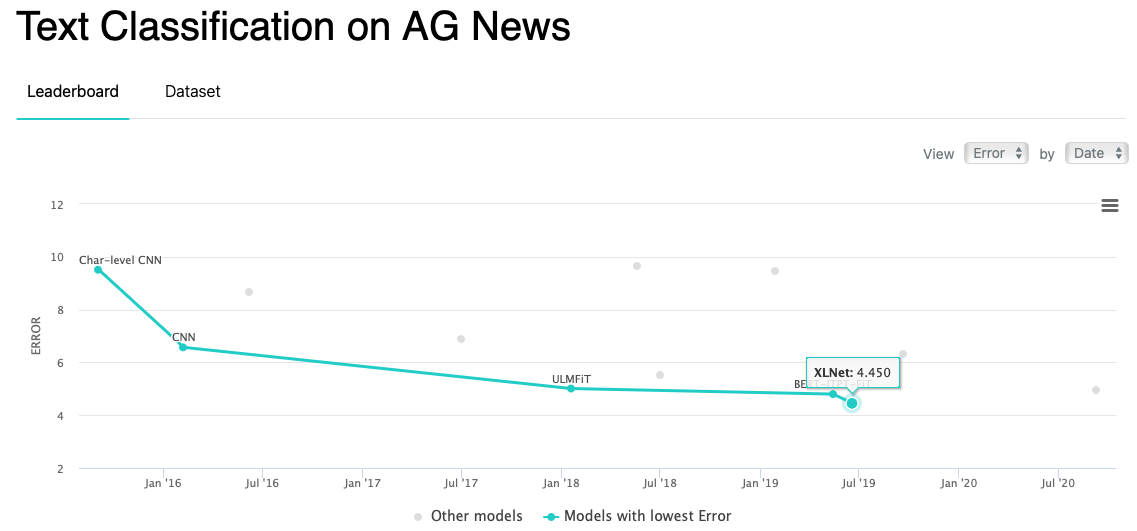
\includegraphics[width=0.8\textwidth]{images/leaderboard.png}
    \caption{我们的错误率为 \textbf{4.57\%},与在 \textbf{32.89B} 数据上训练 \textbf{5.5 天}的 SOTA 模型 \textbf{XLNet} 基本持平(\textbf{4.45\%},0.1\% 属于训练抖动误差范围),明显优于基于传统 LSTM 方法的最优模型 \textbf{L MIXED}(\textbf{4.95\%})}
\end{figure}

模型权重已开源至 \href{https://huggingface.co/Word2Li/LLaMA-3.1-8B-AGNews-SFT}{Hugging Face},项目已开源至 \href{https://github.com/Word2VecT/LLaMA-3.1-8B-AGNews-SFT}{Github}。

\section{实验环境}

\subsection{软件环境}
\begin{itemize}
    \item 操作系统:Linux \texttt{3.10.0-957.el7.x86\_64-x86\_64-with-glibc2.17}
    \item Python 版本:\texttt{3.11.0}
    \item PyTorch 版本:\texttt{2.4.1}
    \item Transformer 版本:\texttt{4.45.2}
    \item DeepSpeed 版本:\texttt{0.15.3}
    \item CUDA 版本:\texttt{1.2.1}
    \item LLaMA-Factory 版本:\texttt{0.9.1.dev0}
\end{itemize}

\subsection{硬件环境}
\begin{itemize}
    \item GPU:NVIDIA A100-SXM4-40GB $\times$ 8
    \item CPU:Intel(R) Xeon(R) Gold 6248R CPU @ 3.00GHz
\end{itemize}

\section{主要实验设计}

文本分类任务的输入为一段文本,输出为该段文本的标签。

根据文本内容与目标的不同,也可以划分为多种任务,例如:新闻分类、情感识别、意图识别等等,对于 Transformer 这些任务在模型的使用上都是类似的。本次实验我们选择了新闻分类任务最难的数据集 \textbf{AG News} 进行实验。

\subsection{Transformer}

Transformer 是一种基于注意力机制的深度学习模型,最初由 Vaswani 等人在 2017 年的论文 \textit{Attention Is All You Need} 中提出。\cite{NIPS2017_3f5ee243}

在之前的序列建模和转换问题中,如语言建模和机器翻译,所采用的主流框架为Encoder-Decoder 框架。传统的 Encoder-Decoder 一般采用 RNN 作为主要方法,基于 RNN 所发展出来的 LSTM 和 GRU 也被曾认为是解决该问题最先进的方法。

但是 RNN(LSTM,GRU)的计算限制为是顺序的,也就是说RNN相关算法只能从左向右依次计算或者从右向左依次计算,这种机制带来了两个问题:\begin{itemize}
    \item 时间片 $t$ 的计算依赖时刻的计算结果,这样限制了模型的并行能力。由于前后隐藏状态的依赖性,无法实现并行,训练动辄数天。
    \item 顺序计算的过程中信息会丢失,尽管LSTM等门机制的结构一定程度上缓解了长期依赖的问题,但是对于特别长期的依赖现象,LSTM依旧无能为力。
\end{itemize}
Transformer 的核心思想是通过注意力机制捕捉输入序列中元素之间的长距离依赖关系。与传统的 RNN 不同,Transformer 完全基于注意力机制,将序列中任意两个位置之间的距离缩小为一个常量,无需依赖序列的顺序处理,大大提高了训练并行度和效率,从而可以广泛应用于自然语言处理(NLP)、计算机视觉(CV)和其他序列建模任务。Transformer 还利用 self-attention 机制实现快速并行,改进了 RNN 最被人诟病的训练慢的缺点,同时也符合现有GPU框架的矩阵化训练。此外,Transformer 可以增加到非常深的深度跳跃连接,充分发掘 DNN 模型的特性,提升模型准确率。

\begin{figure}[htbp]
    \centering
    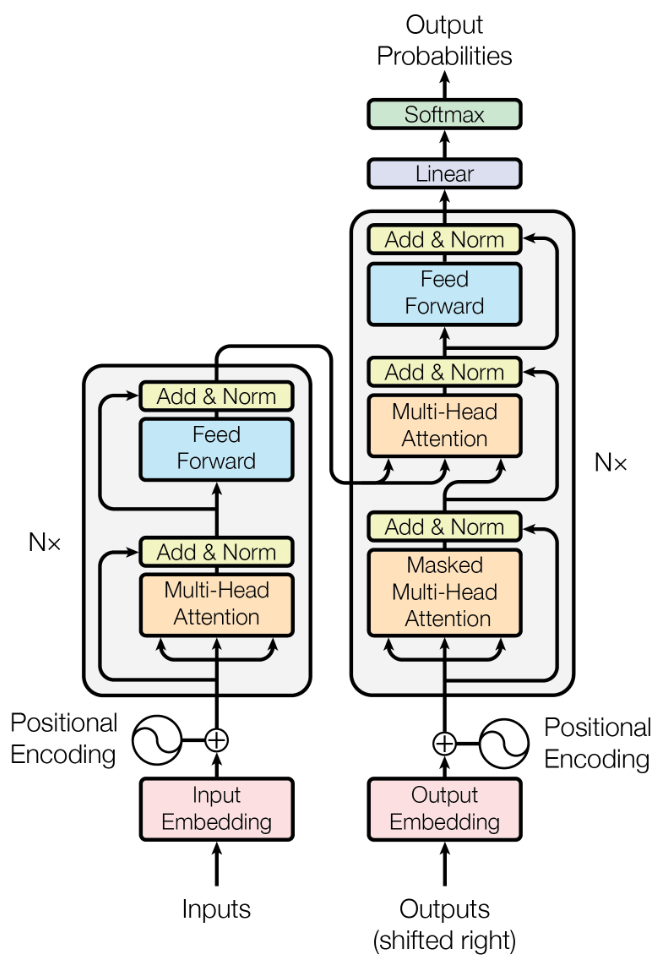
\includegraphics[width=0.5\textwidth]{images/model.png}
    \caption{Transformer 模型架构}
\end{figure}

因此,Transformer 已经完全替代了 RNN 等传统模型,在各类任务上都展示出比传统深度模型更好的效果与潜力,成为了 AI 领域的主流模型。

\subsection{SFT}

最流行的 Transformer LLM 训练流程大概可以分为以下三步:预训练(Pre-Training,PT)、监督微调和 偏好优化(Preference Optimization,PO)。

预训练时,语言模型在超大规模的语料中进行学习,并初步掌握基本的语法规则、逻辑能力、常识知识等等。但是,预训练的目标仅仅是根据上文补全单词,即预测下一个 token,无法使 LLMs 具备对话和问答能力。因此,为了实现更好的与人交互,进一步的训练成为必须。

一种最简单的思路就是 SFT,照搬预训练的目标函数和损失函数进一步微调,但是改变数据的质量和格式。为了使 LLM 对齐人类价值观,我们可以专门筛选一些符合人类价值观的数据;为了让 LLM 适应对话和问答场景,我们可以构造一问一答或者多轮问答的数据。经过上述数据的训练,模型将拟合这部分数据的特性,从而达到我们的目的。用公式表示即:
\[\mathcal{L}_{\text{SFT}} = \mathbb{E}_{\rho_0 \sim \mathcal{D}} \mathbb{E}_{\tau \sim \rho_0} \left[ - \sum_{i=0}^{N} \log T_{\theta}(\pi^*(s_i^*), s_i^*) \right]
\]

本次实验我们选择构建一问一答的单轮对话数据进行 SFT,不涉及 PO。

\subsection{Llama 3.1 8B}

Llama 3.1 是 Meta 今年发布的的大模型系列。一共有 8B,70B,405B 三种参数量版本,为了实验效率与可行性,我们选择 \textbf{8B} 的版本进行实验,并在该模型上进行 SFT。

\textbf{数据}方面,相比前代,Llama 3.1 的数据总量和质量都有所提高,比如对预训练数据更仔细的预处理和管理管道,以及对训练后数据更严格的质量保证和过滤方法。之前的版本 Llama 2 仅在 1.8T token 的数据上进行预训练,而 Llama 3.1 的多语言预训练语料则达到了15.6T token,有超过8倍的增长。符合数据的 Scaling Low。

\textbf{规模}方面,Llama 3.1 的训练使用了超过1.6万个英伟达 H100 GPU,计算总量达到 3.8e25 FLOPS,几乎是 Llama 2 的 50 倍。

为了更好地实现 scale up,Llama 3.1 特别关注了\textbf{复杂度管理},在选择模型架构和算法时,更注重其稳定性和可扩展性。

例如 Llama 3.1 并没有使用最近最受关注的 MoE(Mixture of Experts)架构,而是 decoder-only 架构的稠密 Transformer,仅将原始的 Transformer 架构进行过一些修改和调整,以最大化训练稳定性。类似的做法还有,使用 SFT、RS(Rejection Sampling)、DPO(Direct Preference Optimization)等简洁的训练后流程,而不是更复杂的强化学习算法。

和许多大模型类似,Llama 3.1 的训练也主要包括两个阶段:预训练和后训练。预训练时同样使用``预测下一个 token''作为训练目标,首先将上下文窗口设定为 8K,之后在继续预训练阶段扩展到 128K。后训练阶段通过多个轮次迭代的人类反馈来改进模型,显著提升模型在特定下游任务的能力。

\subsubsection{模型架构}

Llama 3.1 依旧使用标准的稠密 Transformer,与之前的系列 Llama 和 Llama 2 在架构方面并没有显著差异,性能的改进主要来自训练数据质量、多样性的提升,以及规模扩展。
\begin{figure}[htbp]
    \centering
    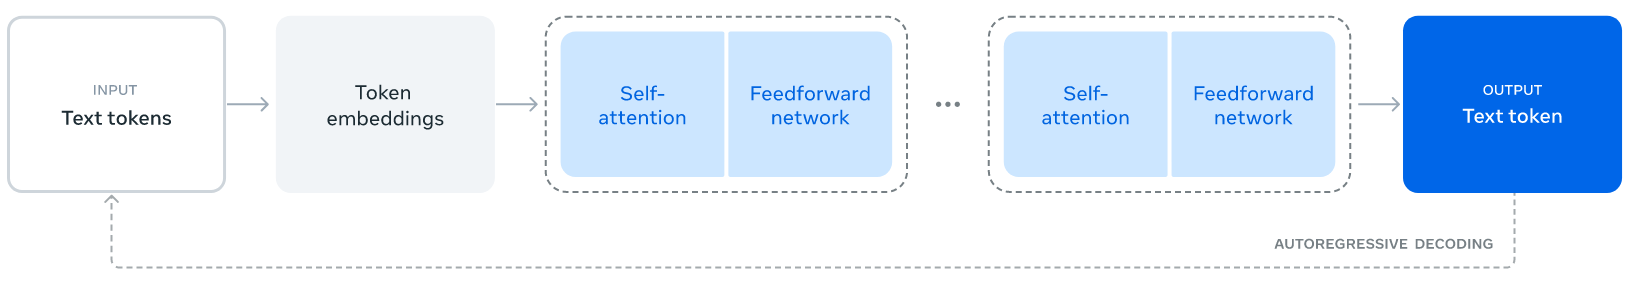
\includegraphics[width=0.8\textwidth]{images/architecture.png}
    \caption{Llama 3.1 整体架构和训练示意图}
\end{figure}

相较于传统的 Transformer,Llama 3.1 的架构有以下改进:\begin{itemize}
    \item 分组查询注意力(GQA):带有8个键-值头,提升推理速度并减少解码时的KV缓存。
    \item 注意力掩码:防止同一序列中不同文档之间出现自注意力。这个技巧在标准预训练中效果有限,但对很长的序列进行继续预训练时非常重要。
    \item 128K token 词表:包括 tiktoken 中的 100K 以及额外的 28K,以更好支持非英语语言。与 Llama 2 相比,同时提高了英语和非英语的压缩比率。
    \item 将 RoPE(Rotary Position Embedding)的超参数 $\theta$ 设置为500000:更好支持长上下文
\end{itemize}

对于 8B 的模型,共有 32 层 Transformer,模型纬度为 4096,注意力头数为 32,前馈网络纬度为 14336,峰值学习率为 $3\times10^{-4}$,激活函数选择了 SwiGLU。

\subsection{LLaMA-Factory}

大模型开发,存在许多训练框架来加速和方便我们的训练过程,如 DeepSpeed、LLaMA-Factory,Meta Lingua,Unsloth 等,我们选择了 \textbf{LLaMA-Factory} 来进行实验。\cite{zheng2024llamafactory}

LLaMA-Factory(Large Language Model Factory)支持多种预训练模型和微调算法,提供了一套完整的工具和接口,使得用户能够轻松地对预训练的模型进行定制化的训练和调整,以适应特定的应用场景,如文本分类、智能客服、语音识别、机器翻译等。\begin{itemize}
    \item 支持的模型:LLaMA-Factory 支持多种大型语言模型,包括但不限于 \textbf{LLaMA}、LLaVA、Mistral、Mixtral-MoE、Qwen、Yi、Gemma、Baichuan、ChatGLM、Phi 等等。
    \item 集成方法:包括(增量)预训练、(多模态)\textbf{指令监督微调}、奖励模型训练、PPO 训练、DPO 训练、KTO 训练、ORPO 训练等等多种方法。
    \item 运算精度与优化算法:提供 \textbf{16 比特全参数微调}、冻结微调、LoRA 微调和基于 AQLM/AWQ/GPTQ/LLM.int8/HQQ/EETQ 的 2/3/4/5/6/8 比特 QLoRA 微调等多种精度选择,以及 GaLore、BAdam、DoRA、LongLoRA、LLaMA Pro、Mixture-of-Depths、LoRA+、LoftQ 和 PiSSA 微调等先进算法。
    \item 支持 \textbf{FlashAttention-2} 和 Unsloth 加速算子,支持 Transformers 和 vLLM 推理引擎,以及支持 LlamaBoard、TensorBoard、\textbf{Wandb}、MLflow 等等实验面板。
\end{itemize}

\begin{figure}[htbp]
    \centering
    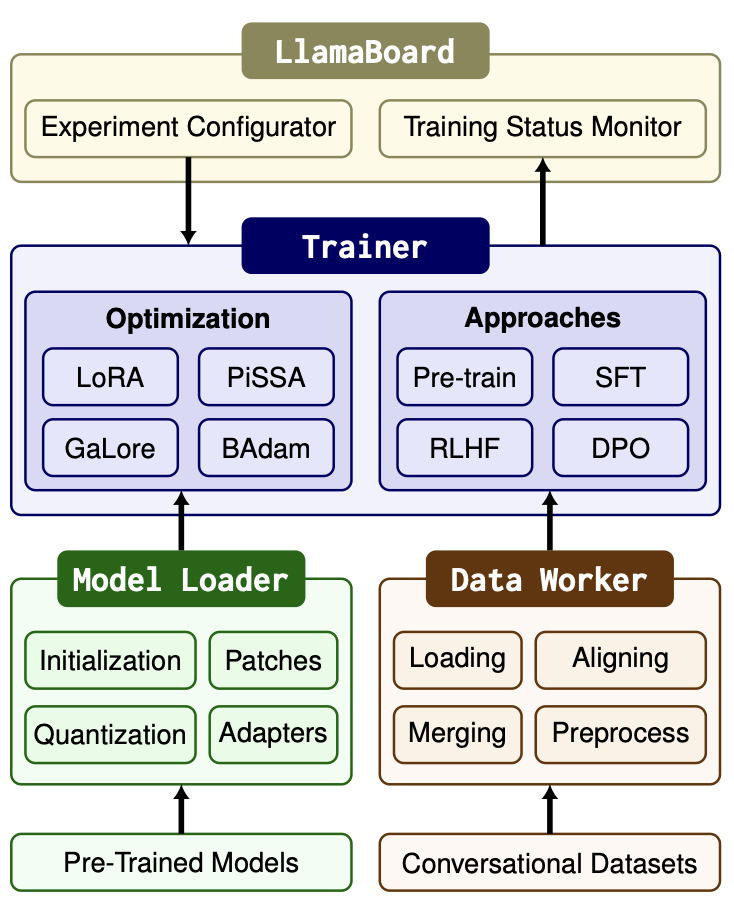
\includegraphics[width=0.5\textwidth]{images/factory.png}
    \caption{LLaMA-Factory 整体架构}
\end{figure}

虽然上述很多功能在实验都没有涉及,但是 LLaMA-Factory 仍然为我们提供了很多便利。

\section{具体实验过程}

\subsection{数据集选择}

\href{http://groups.di.unipi.it/~gulli/AG_corpus_of_news_articles.html}{AG 语料库}是一个包含超过100万篇新闻文章的集合。这些新闻文章是由ComeToMyHead在超过1年的时间里从2000多个新闻来源收集而来的。ComeToMyHead是一个自2004年7月以来运行的学术新闻搜索引擎。

该数据集由学术界提供,供数据挖掘(聚类、分类等)、信息检索(排名、搜索等)、XML、数据压缩、数据流等任何其他非商业活动的研究用途。

AG News 选择了这个语料库中的四个最大类别(World、Sports、Business、Sci/Tech)来构建数据集,仅使用标题和描述字段。每个类别的训练样本数量为30000,测试样本为1900。总的数据量为训练集120000,测试集7600。

\begin{table}[htbp]
    \centering
    \begin{tabular}{cccc}
        \toprule
        \textbf{类别} & \textbf{训练集} & \textbf{测试集} & \textbf{占比} \\
        \midrule
        World & 30000 & 1900 & 25\% \\
        Sports & 30000 & 1900 & 25\%  \\
        Business & 30000 & 1900 & 25\% \\
        Sci/Tech & 30000 & 1900 & 25\%  \\
        \midrule
        总计 & 120000 & 7600 & 100\%  \\
        \bottomrule
    \end{tabular}
    \caption{AG News 数据集}
\end{table}

\subsection{数据预处理}

我们可以直接从 \href{https://huggingface.co/datasets/SetFit/ag_news}{Hugging Face} 或者 \href{https://www.kaggle.com/datasets/amananandrai/ag-news-classification-dataset}{kaggle} 上下载数据集。

\begin{figure}[htbp]
    \centering
    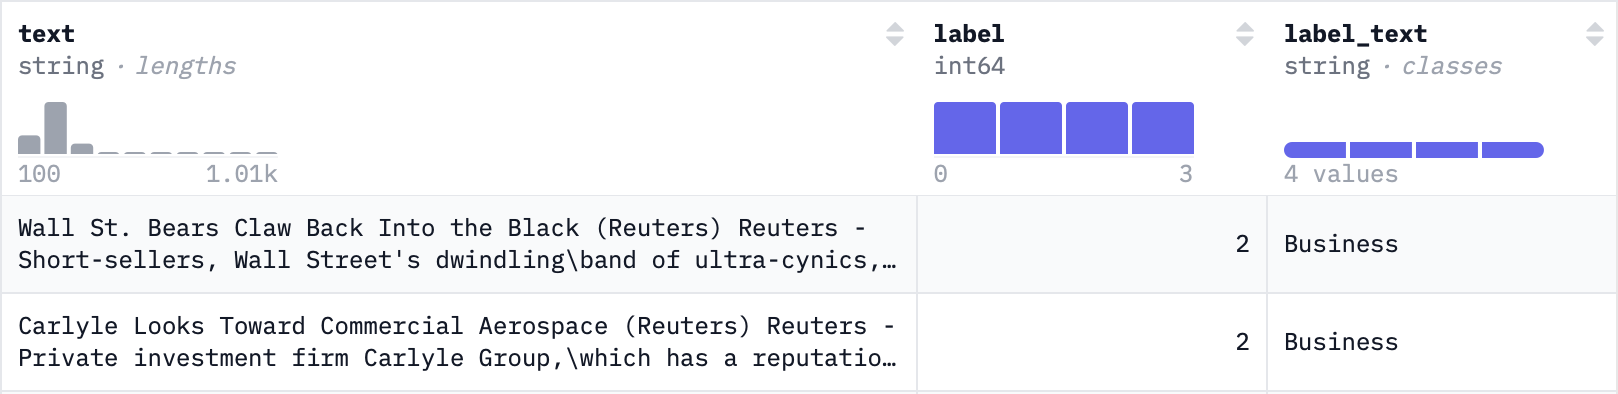
\includegraphics[width=0.8\textwidth]{images/orgin_title.png}
    \caption{AG News 原始数据示例}
\end{figure}

我们从 Hugging Face 上下载了 jsonl 文件的数据集,原始数据集的对象名称为\texttt{text}、\texttt{label} 和 \texttt{label\_text},该格式不能直接用于训练,我们编写脚本对数据集进行了预处理,得到能够直接训练的统一格式数据,处理后的 jsonl 文件包含对象名称为 \texttt{id}、\texttt{instruction}、\texttt{input} 和 \texttt{output}。对于特殊符号,我们采用 \texttt{ensure\_ascii=False} 防止 JSON 编码字符串时出现 Unicode 的转义序列,而是通过在特殊字符前面添加 \textbackslash 来表示。

\begin{figure}[htbp]
    \centering
    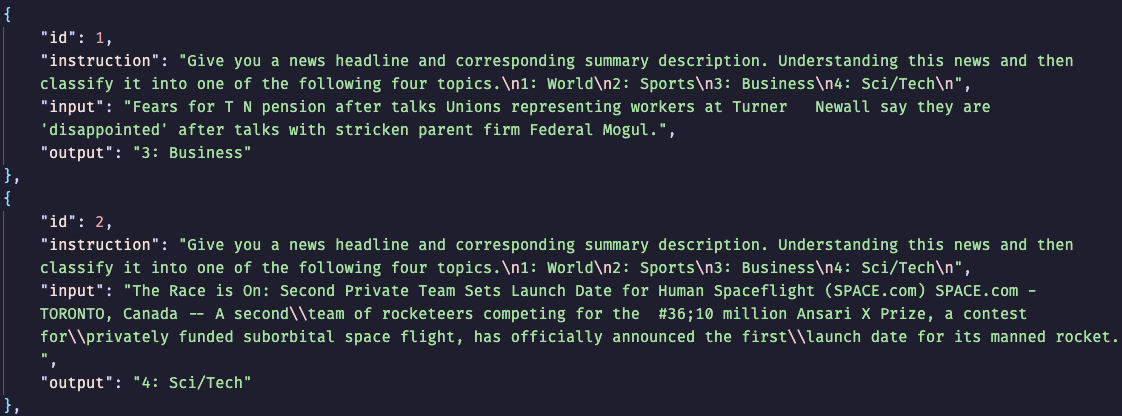
\includegraphics[width=0.8\textwidth]{images/preprocessed_title.png}
    \caption{AG News 预处理后数据示例}
\end{figure}

其中 \texttt{id} 为顺序分配的序列号,便于后续定位数据进行分析, \texttt{instruction} 是我们为大模型设置的 Prompt, 这个将在后面详细讨论,\texttt{input} 对应原来的 \texttt{text} 即新闻的内容,\texttt{output} 对应原来的 \texttt{label} 和 \texttt{label\_text} 即分类预测输出结果。 

去\textbf{停用词}是 NLP 中的一种常见预处理步骤,指从文本中移除对特定任务无关或贡献较小的高频词汇。而对于大模型推理而言,介于 Transformer 的强上下文推理能力,不需要去停用词,此外,停用词可能携带重要的语义和上下文信息,在文本分类任务中,停用词有助于模型理解句法结构和语义关系。大模型能够通过其强大的表示能力和注意力机制自动判断哪些词对任务重要,因此人工去除停用词反而可能丢失关键信息,影响模型性能。因此无需进行去停用词操作。

\subsubsection{Prompt 设置}

Prompt 特指用于触发和引导人工智能语言模型生成特定输出的文本或语句片段。在使用 LLM 时,用户会提供一个简短的提示作为 prompt,然后模型根据这个提示生成相应的文本。

Prompt 的内容可以是问题、描述、关键词、上下文等,用来引导模型产生特定主题或内容的文本。例如 ``讲个笑话''、``用 Python 编个贪吃蛇游戏'' 等。这些指令可以是单词、短语、问题或完整的句子,用于指导模型生成特定的回答、文本、摘要或其他输出,本质上就是用户发给大模型的指令。

因此提示工程也叫指令工程(Prompt Engineering),提示工程是指设计和构建用于指导大语言模型生成文本的有效 prompt 的过程。Prompt 就是使用自然语言把问题描述清楚的一种能力。

针对本次的任务,我们需要引导大模型对新闻进行分类,因此设置的 Prompt 为:\begin{textcode}
    Give you a news headline and corresponding summary description. Understanding this news and then classify it into one of the following four topics.
    1: World
    2: Sports
    3: Business
    4: Sci/Tech
\end{textcode}

Prompt 的设置对大模型的训练和后续表现非常重要,一个好的 prompt 可以提高模型的准确率和泛化能力,因此我们可以多次设置 prompt 进行修改并测试,在后续将会详细介绍这一点。设置的 Prompt 作为训练数据的 \texttt{instruction}。

\subsubsection{分词与文本向量化}

分词是自然语言处理中的一个重要步骤,将文本数据转换为模型可以理解的数据。在大模型训练中,大多数分词器都以两种风格提供:一种是完整的 Python 实现,另一种是基于 Rust 库 Tokenizers 的 ``Fast'' 实现,优势在于支持多线程,可以更好地利用多核 CPU 的性能,可以显著提升速度,特别是在批处理分词时,使用``Fast''实现可以获得显著的速度提升。此外 Fast Tokenizer 还提供了额外的方法,用于在原始字符串(字符和单词)与标记空间之间进行映射。例如,可以获取包含给定字符的标记的索引,或获取与给定标记对应的字符范围。在本次实验中,我们使用了 \textbf{Fast Tokenizer} 进行分词。

通过将文本序列转化为数字序列也就是 token 编号,这样就可以得到 Transfomer 的输入,每一个 token 都会对应一个 id,根据 id,可以找到 word embedding,这样便将文本输入变成了大模型能够理解的向量,而大模型的学习便是对这些 word embedding 进行更新。

值得注意的是,在 Transformer 大模型训练时,我们采用的是 BPE(Byte Pair Encoding)分词算法,即将 subword 作为分词的单元而不是整个单词,这样可以大大减少词表的大小,同时还能够充分表达含义。

分词示例如~\autoref{fig:token}:\begin{figure}[htbp]
    \centering
    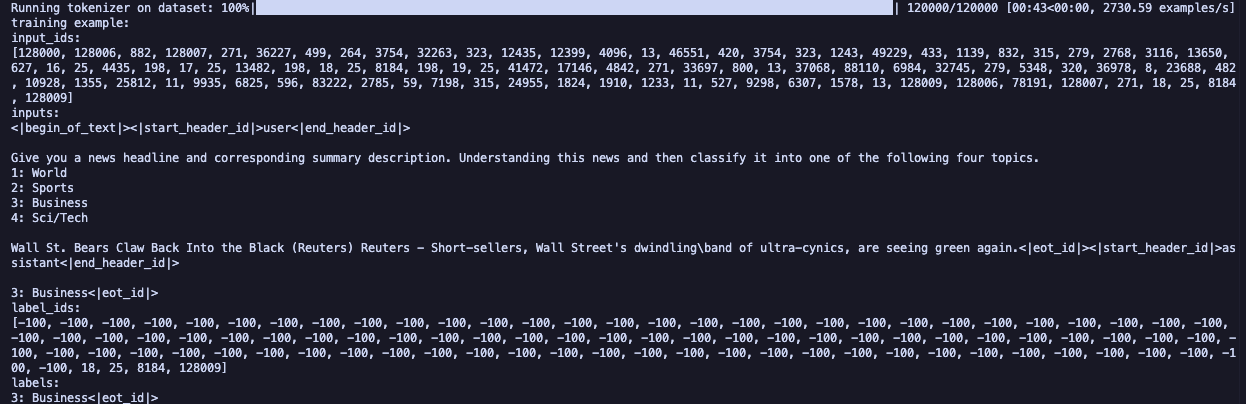
\includegraphics[width=0.8\textwidth]{images/token.png}
    \caption{分词示例}
    \label{fig:token}
\end{figure}

由于在预训练阶段,已经完成了对词表的构建,因此在微调阶段,我们可以直接使用预训练的词表,不需要再次进行词频统计构建词表操作。

\subsection{训练}

\subsubsection{超参数选择以及配置}

对于参数选择与模调优,大模型对超参数的设置较为鲁棒,我们具体的研究过程参见~\autoref{sec:exp}。

由于对于大模型来说,与与训练不同,SFT 阶段在于学习特定任务的特征,并且文本分类任务对于大模型来说较为简单,因此我们学习率不用设置的过高,较低的学习率可以防止过拟合,我们将\textbf{学习率}设置为 $2\times10^{-5}$。我们也对不同的学习率进行了测试。

但由于在初始阶段直接使用较高的学习率可能导致不稳定性,使得权重更新幅度过大。我们设置 \textbf{Warmup 阶段},可以让学习率从较小的值开始,逐渐增加到预设的峰值,之后再按照学习率调度策略降低。我们设置了 \textbf{Cosine Scheduler} 逐步降低学习率,使其在训练后期逐渐接近零,从而帮助模型在接近最优解时更加稳定。

我们将每个设备上的\textbf{训练批次大小}设置为 4,总共 8 卡,因此总的批次大小为 32。批次大小表示在一块 GPU 上一次前向传播和后向传播中处理的样本数量。批次大小越大,显存占用越多。较大的批次通常使梯度更新更加平稳,但可能需要更大的学习率来获得最佳结果。同时设置\textbf{梯度累积步数}为 8,表示表示经过多次8次前向传播后,累积的梯度再进行一次后向传播(权重更新),这样可以通过累积多个小批次的梯度,模拟大批次的训练效果,而不需要占用额外显存,从而降低显存需求。但是由于我们的显卡资源比较充裕,这样的设置稍微有点保守,但影响不大。

由于 8B 模型的参数也不是很小,因此是无法在一台 A100 上进行训练的,我们通过使用 \textbf{Flash Attention 2},通过高效的注意力计算实现,基于数学重构和内存优化,使用了现代 GPU 上的 chunking 和分块计算技术,从而降低标准注意力计算显存调用,提高计算效率。同时还使用微软开发的 \textbf{DeepSpeed} 库,并采用 ZeRO-3 参数分布(Parameter Partitioning)从而可以在多个 GPU 上分布式进行训练,加速训练过程,使训练变得可能。

综上,我们最终使用的参数如下:\begin{textcode}
torchrun --nnodes=1 --nproc-per-node=8 src/train.py \
    --deepspeed examples/deepspeed/ds_z3_config.json \
    --stage sft \
    --do_train \
    --use_fast_tokenizer \
    --flash_attn fa2\
    --model_name_or_path /mnt/petrelfs/tangzinan/LLaMA-Factory/models/LLama3.1-8B \
    --dataset ag_news_train \
    --template llama3 \
    --finetuning_type full \
    --output_dir saves/LLama3.1-8B/full/train_2024-12-03-21-04-03 \
    --overwrite_cache \
    --overwrite_output_dir \
    --warmup_ratio 0.03 \
    --weight_decay 0. \
    --per_device_train_batch_size 4 \
    --gradient_accumulation_steps 4 \
    --ddp_timeout 9000 \
    --learning_rate 2e-5 \
    --lr_scheduler_type cosine \
    --cutoff_len 4096 \
    --save_steps 2000 \
    --logging_steps 1 \
    --plot_loss \
    --resize_vocab \
    --num_train_epochs 1 \
    --bf16 \
    --report_to wandb \
    --run_name llama3.1-8B-agnews-steps4
\end{textcode}

\subsubsection{核函数}

核函数是机器学习中用来衡量两个输入之间相似度的函数,常用于 SVM、核回归等模型中。核函数 \( k(x, x') \) 等价于隐空间中内积:
  \[
  k(x, x') = \phi(x) \cdot \phi(x')
  \]
  其中,\(\phi\) 是映射函数,将输入数据从原空间映射到高维隐空间。

  在 Transformer 的自注意力机制中,点积注意力(Dot Product Attention)是核心:
  \[
  \text{Attention}(Q, K, V) = \text{softmax}\left(\frac{QK^T}{\sqrt{d_k}}\right)V
  \]
  其中:\begin{itemize}
    \item \( Q \) 是查询(Query)向量。
    \item \( K \) 是键(Key)向量。
    \item \( V \) 是值(Value)向量。
  \end{itemize}

这里的点积 \( QK^T \) 实际上计算了查询与键的相似度,可以看作是\textbf{核函数的隐式形式},即一个\textbf{线性核}。

虽然我们使用的 LLM 没有直接显式地使用核函数,但其核心机制(尤其是注意力机制)可以看作是隐式的核函数应用,特别是点积注意力等效于一个线性核函数。

\subsubsection{推理及训练过程}

为了便于观察实验现象,跟踪实验,我们采用了 \textbf{WandB} 面板进行实验的监控和记录,通过配置 WandB,可以自动记录训练期间的指标(如损失、准确率、学习率等),可视化模型训练曲线、模型参数变化和调优过程。

比如,我们可以查看训练的实时结果曲线,包括损失函数下降、学习率变化等。从而对实验结果进行直观分析。此外还支持多实验对比,从而帮助我们选择超参数。

对于本次实验,WandB 面板信息如图~\autoref{fig:wandb}:\begin{figure}[htbp]
    \centering
    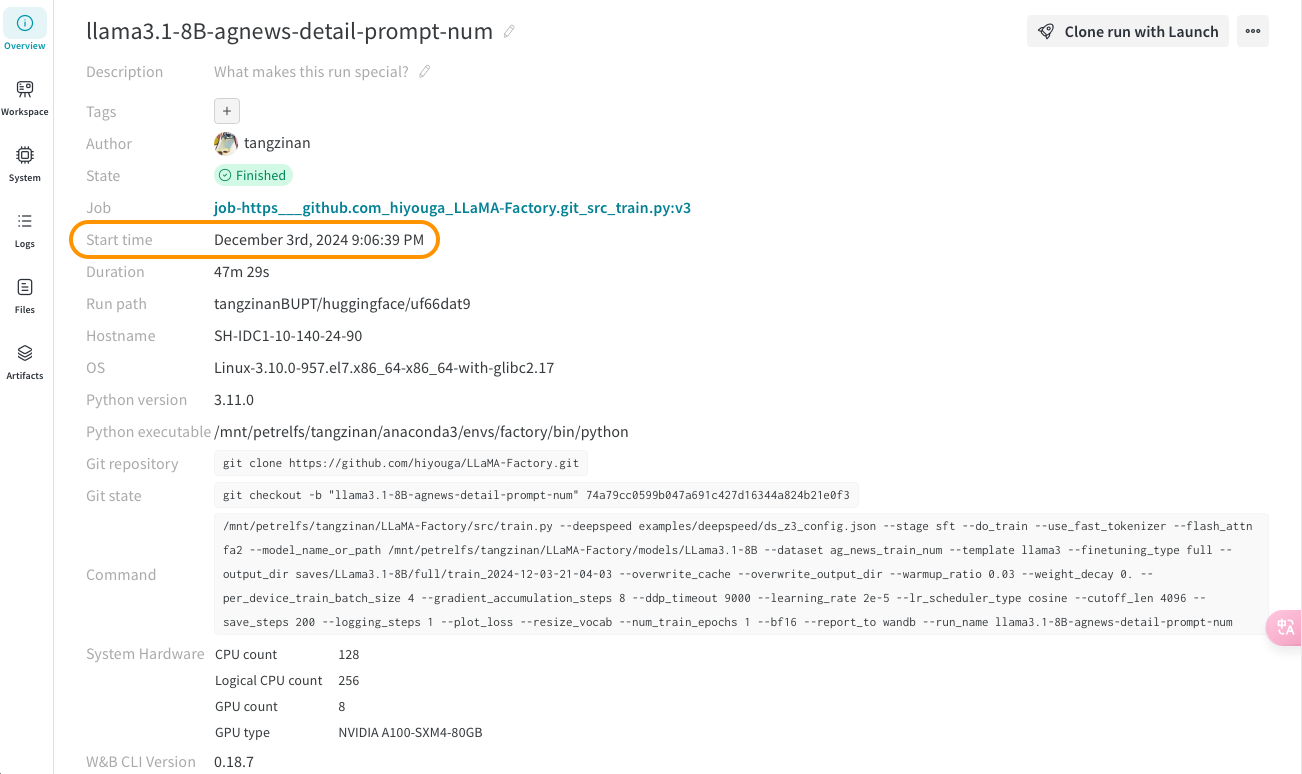
\includegraphics[width=0.8\textwidth]{images/wandb.png}
    \caption{WandB 面板信息(带有时间信息)}
    \label{fig:wandb}
\end{figure}

训练过程变化曲线如图~\autoref{fig:train}:\begin{figure}[htbp]
    \centering
    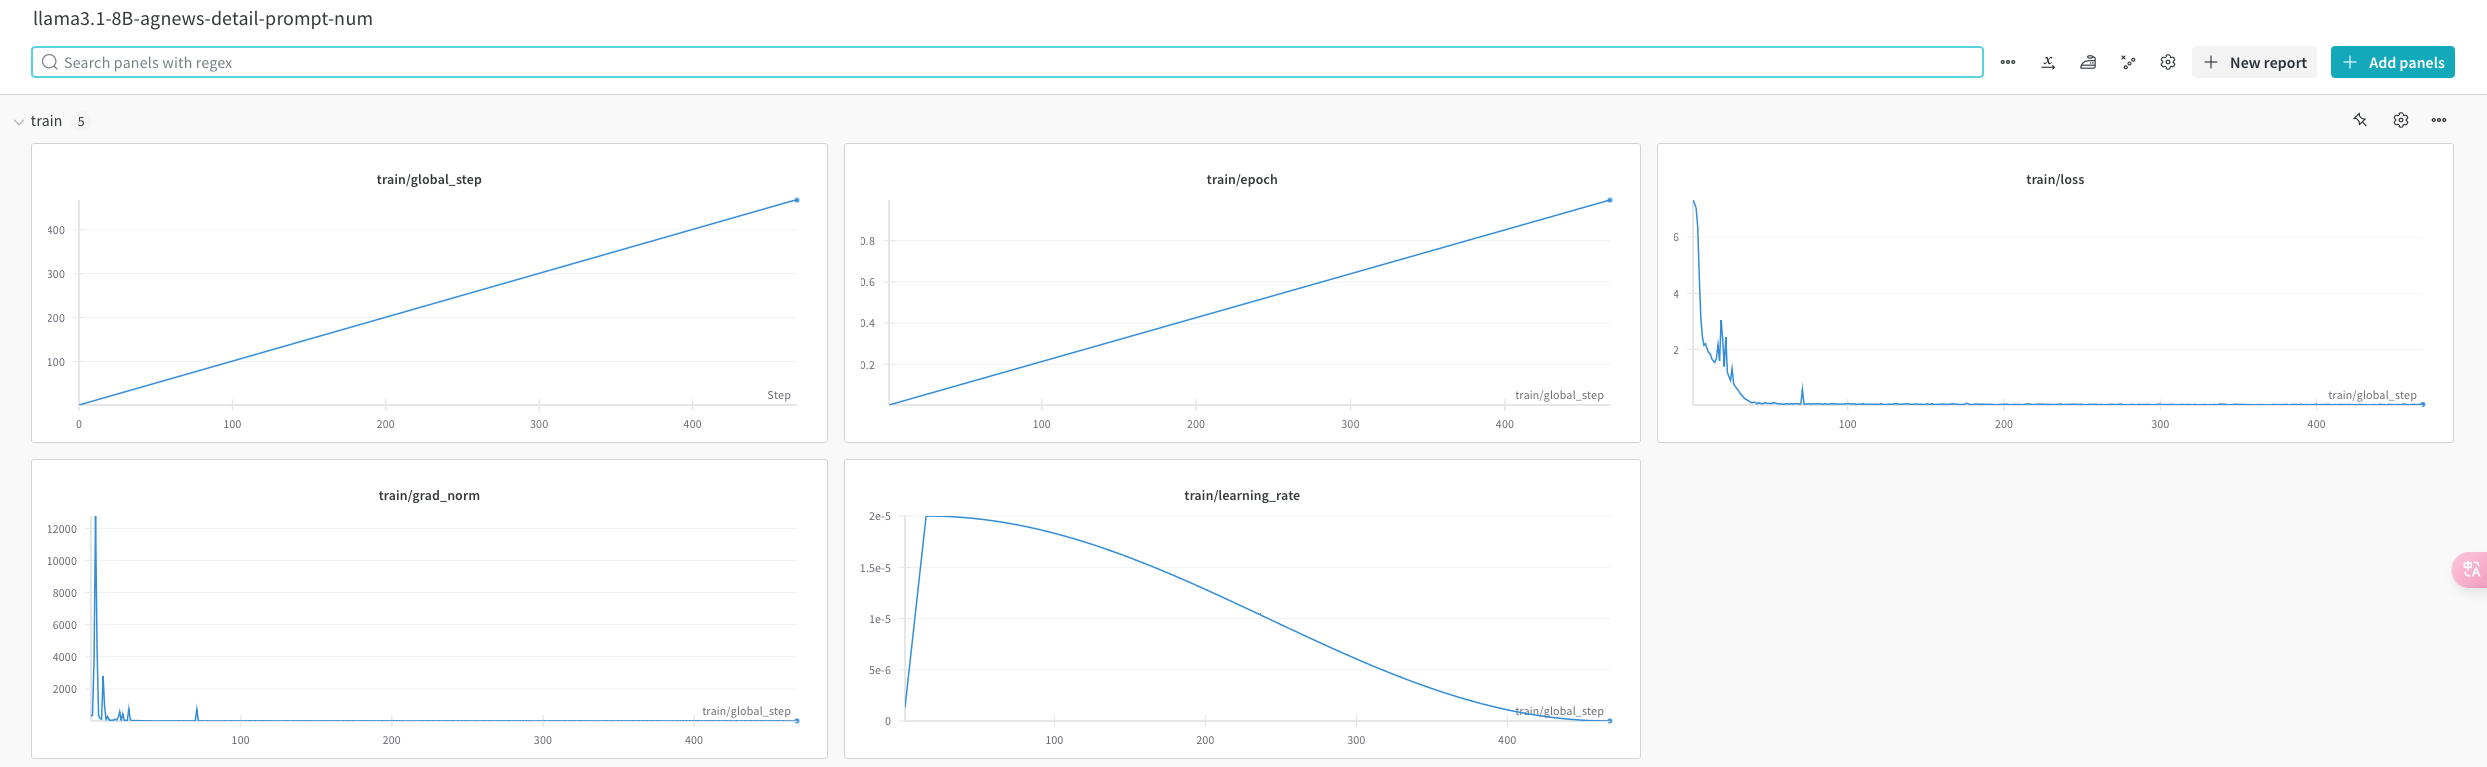
\includegraphics[width=0.8\textwidth]{images/board.png}
    \caption{训练过程变化曲线总览}
    \label{fig:train}
\end{figure}

可以见到,由于分类任务对于现代大模型来说较为简单,模型在微调训练过程中很快就收敛到了一个较好的状态,损失函数下降较快,准确率较高。损失的变化具体如~\autoref{fig:loss} 所示。\begin{figure}[htbp]
    \centering
    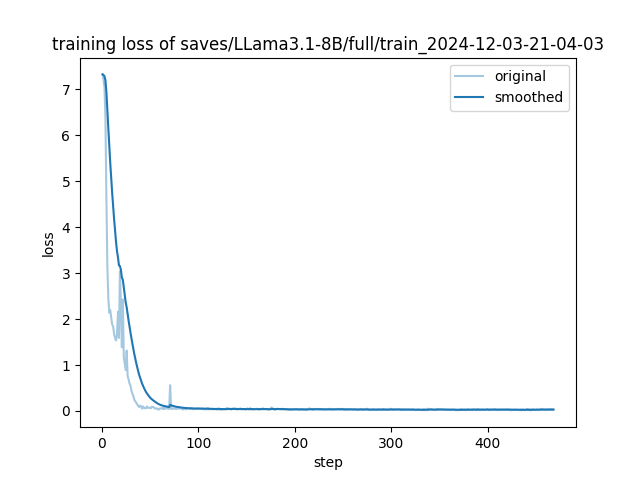
\includegraphics[width=0.8\textwidth]{images/loss.png}
    \caption{损失变化曲线}
    \label{fig:loss}
\end{figure}

\subsection{测试}

为了测试分类准确度,我们需要得到微调后的模型在测试集上的推理 inference 结果,然后与测试集 label 进行对比,计算准确率。

对于测试,我们仍然使用 LLaMA-Factory,通过设置推理 yaml 脚本,在测试机上进行 8 卡批量推理,加快效率。

yaml 脚本设置如下:\begin{yamlcode}
    ### model
    model_name_or_path: /mnt/petrelfs/tangzinan/LLaMA-Factory/saves/LLama3.1-8B/full/train_2024-12-03-21-04-03
    
    ### method
    stage: sft
    do_predict: true
    finetuning_type: full
    
    ### dataset
    eval_dataset: ag_news_test
    template: llama3
    cutoff_len: 4096
    max_samples: 100000
    overwrite_cache: true
    preprocessing_num_workers: 16
    
    ### output
    output_dir: /mnt/petrelfs/tangzinan/LLaMA-Factory/news_train/llama/final
    overwrite_output_dir: true
    
    ### eval
    per_device_eval_batch_size: 1
    predict_with_generate: true
    ddp_timeout: 180000000
\end{yamlcode}

参数的设置与训练脚本参数都是对应的,在这里不过多赘述。值得注意的是 \texttt{preprocessing\_num\_workers} 应适当调大,防止分词等预处理的速度跟不上GPU的推理速度。推理过程如图~\autoref{fig:eval}:\begin{figure}[htbp]
    \centering
    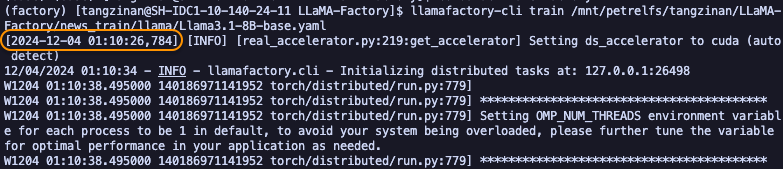
\includegraphics[width=0.8\textwidth]{images/inference.png}
    \caption{测试过程(带有时间信息)}
    \label{fig:eval}
\end{figure}

推理结束后,我们可以得到对于每个 test 集的数据,得到模型的输出,如~\autoref{fig:output}:\begin{figure}[htbp]
    \centering
    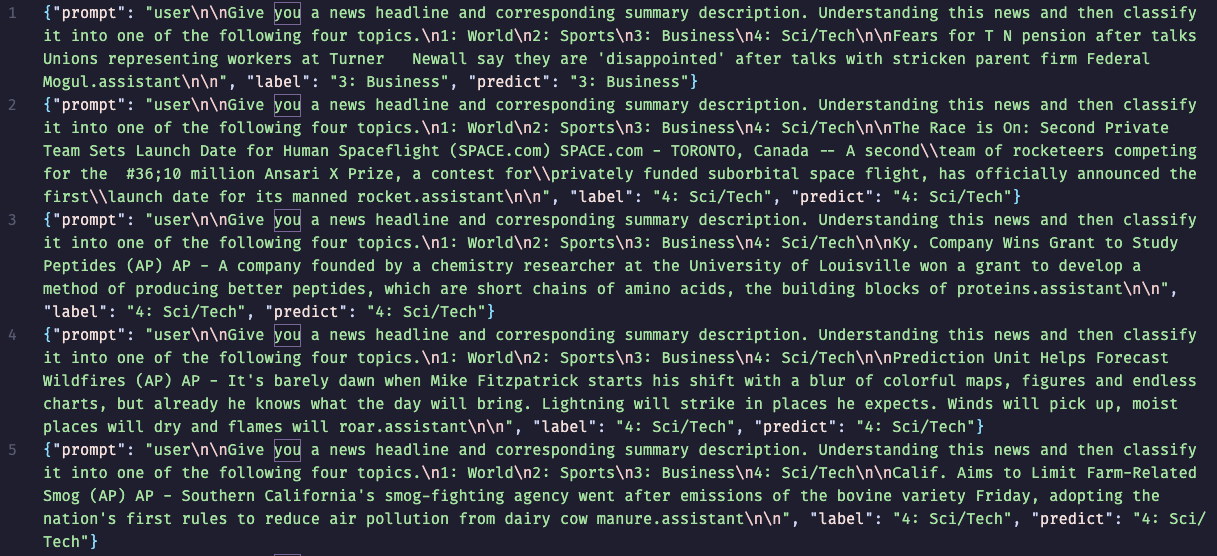
\includegraphics[width=0.8\textwidth]{images/infer.png}
    \caption{测试输出结果示例}
    \label{fig:output}
\end{figure}

随后便能够通过 evaluation 脚本,得到模型的性能。

\subsection{实验结果}

\subsubsection{评测数据}

通过 evaluation 脚本,对分类结果的准确率、精确率、召回率、和 F1 Score 进行计算,得到实验结果如~\autoref{fig:res}所示。\begin{figure}[htbp]
    \centering
    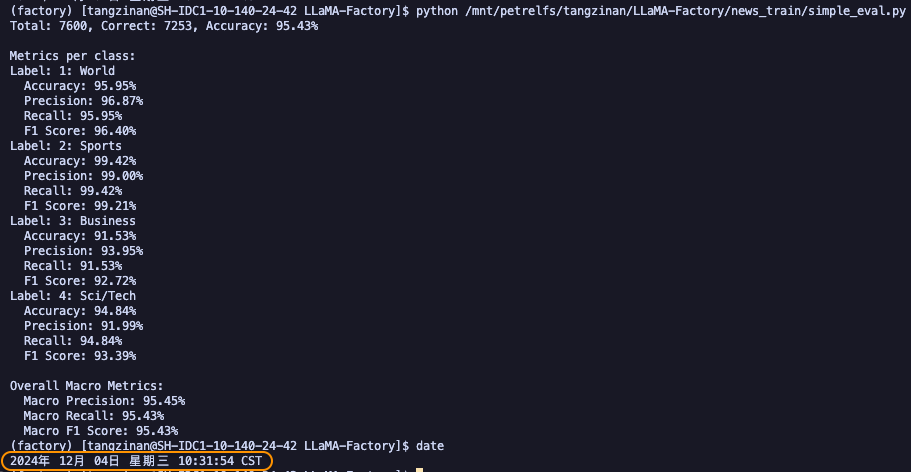
\includegraphics[width=0.8\textwidth]{images/eval.png}
    \caption{测试结果(带有时间信息)}
    \label{fig:res}
\end{figure}

得到的评测结果表格如~\autoref{tab:res}:

\begin{table}[htbp]
    \centering
    \begin{tabular}{ccccc}
        \toprule
        分类 & 准确率 & 精确率 & 召回率 & F1 Score \\
        \midrule
        World & 95.95\% & 96.87\% & 95.95\% & 96.40\% \\
        Sports & 99.42\% & 99.00\% & 99.42\% & 99.21\% \\
        Business & 91.53\% & 93.95\% & 91.53\% & 92.72\% \\
        Sci/Tech & 94.84\% & 91.99\% & 94.84\% & 93.39\% \\
        \textbf{总体(宏平均)} & \textbf{95.43\%} & \textbf{95.45\%} & \textbf{95.43\%} & \textbf{95.43\%} \\
        \bottomrule
    \end{tabular}
    \caption{测试结果表格}
    \label{tab:res}
\end{table}

可以看出,对 Sports 的分类效果最好,这可能是因为 Sports 的新闻往往有着明显的特征,而 Business 的分类效果相对较差,这可能是因为 Business 的新闻往往涉及到更多的细节和背景知识,对模型的要求更高,此外 Business 的定义比较广阔,可能会有一些边界情况混淆。

同时画出混淆矩阵如~\autoref{fig:confusion}所示:\begin{figure}[htbp]
    \centering
    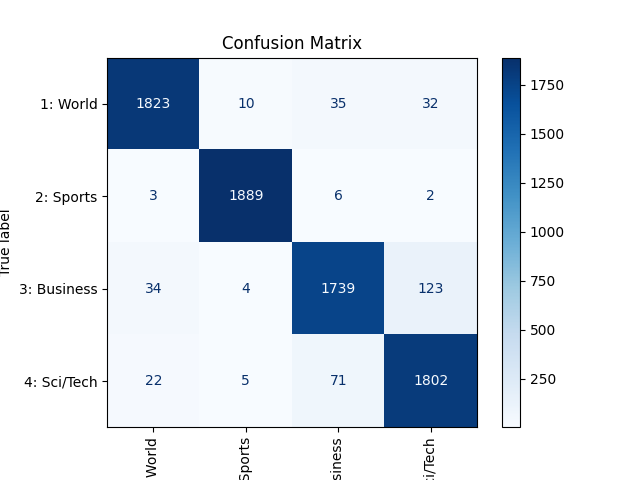
\includegraphics[width=0.8\textwidth]{images/matrix.png}
    \caption{混淆矩阵}
    \label{fig:confusion}
\end{figure}

结果可以看到,模型容易将 Business 和 Sci/Tech 的分类弄混,这可能是因为这两个类别的新闻有一些相似的特征,比如都涉及到技术、商业等方面的内容,但是 Sci/Tech 的新闻可能更加偏向于技术和科学,而 Business 的新闻可能更加偏向于商业和经济,模型没有很好识别出这一点。

\subsection{分类结果可视化}

由于得到的 word embedding 是高维度的,使用 TSNE 进行降维可视化,将高维数据映射到二维平面上,以便于观察分类结果。

label 的分布如~\autoref{fig:label}:\begin{figure}[htbp]
    \centering
    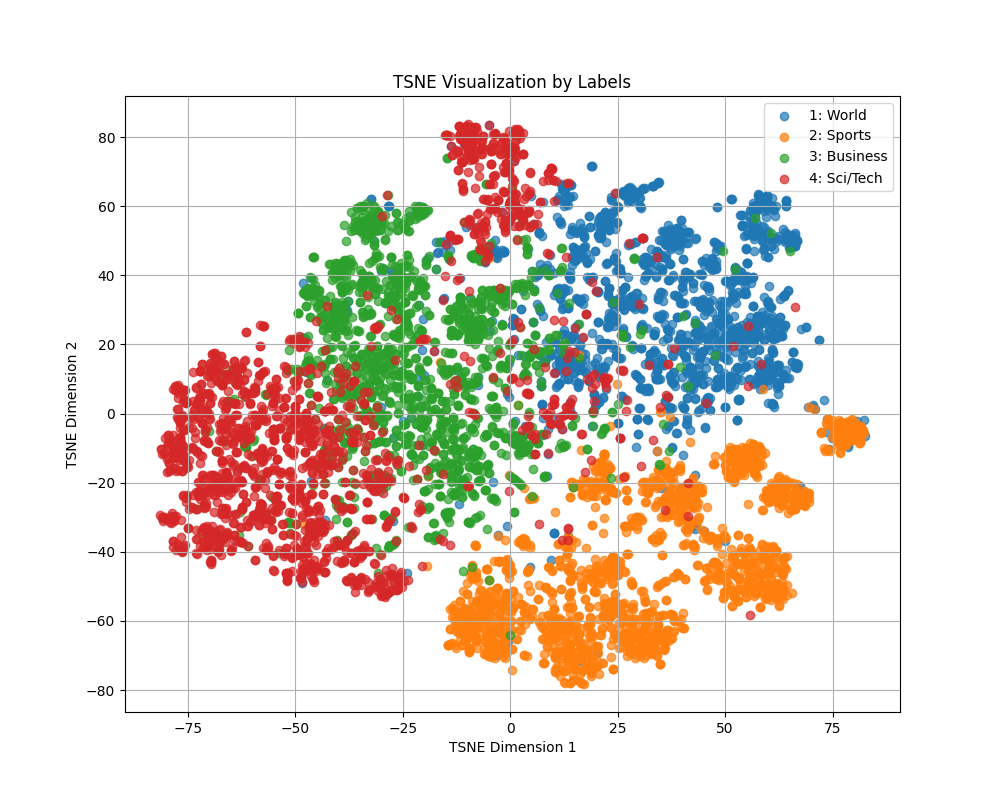
\includegraphics[width=0.7\textwidth]{images/label_tsne.png}
    \caption{label 分布}
    \label{fig:label}
\end{figure}

分类结果分布如~\autoref{fig:res_tsne}:\begin{figure}[htbp]
    \centering
    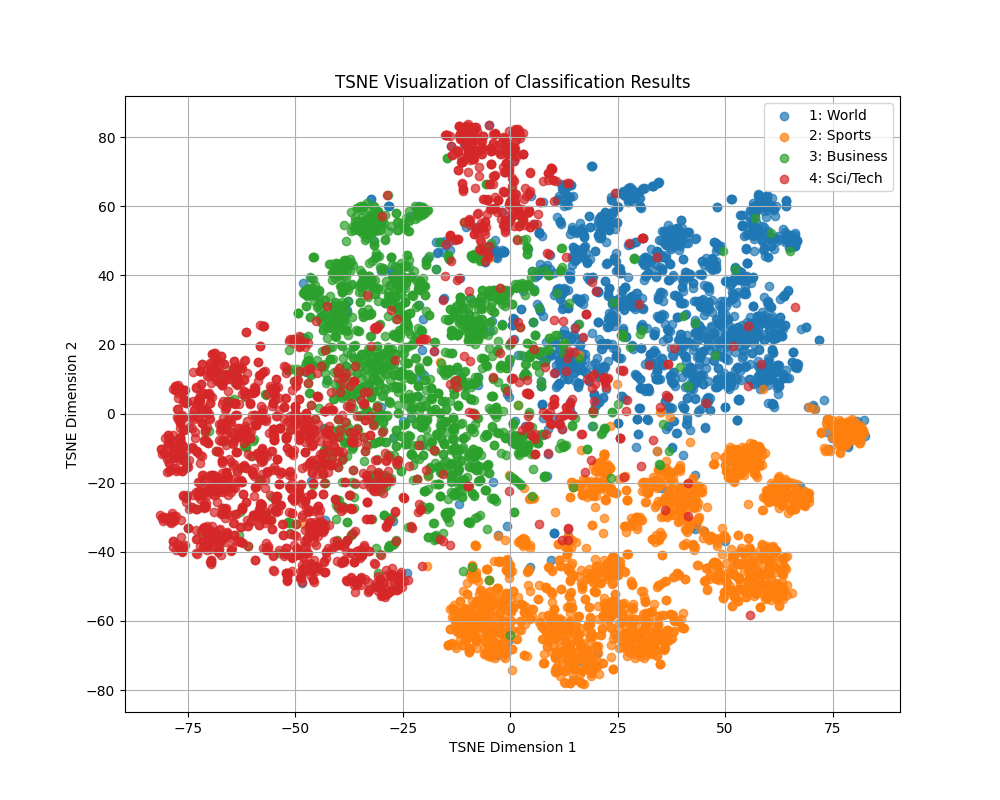
\includegraphics[width=0.7\textwidth]{images/classification_tsne.png}
    \caption{分类结果分布}
    \label{fig:res_tsne}
\end{figure}

为了便于观察,我们将错误的分类标出,如~\autoref{fig:wrong}:\begin{figure}[htbp]
    \centering
    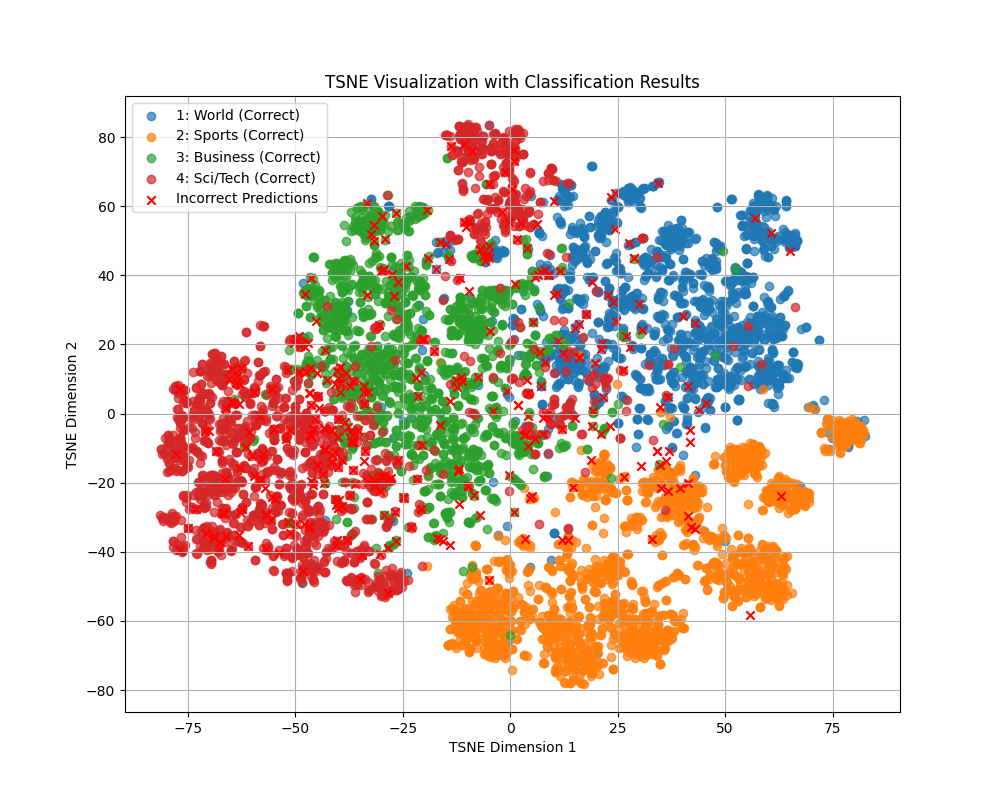
\includegraphics[width=0.7\textwidth]{images/classification_tsne_with_incorrect.png}
    \caption{错误分类}
    \label{fig:wrong}
\end{figure}

这也进一步证明了我们的准确率情况,Sports 类的簇较为独立,因此分类效果很好,Business 甚至有两个簇,因此效果最差,此外,Business 和 Sci/Tech 的簇重叠较大,因此二者容易混淆。

\subsubsection{调参经历} \label{sec:exp}

本次实验中,我们对学习率、梯度累积步数、训练步数以及 Prompt 等参数进行了调整,以观察对模型性能的影响。

\begin{figure}[htbp]
    \centering
    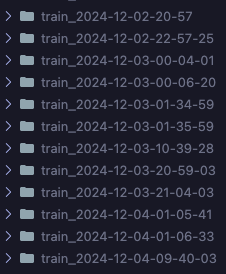
\includegraphics[width=0.3\textwidth]{images/save.png}
    \caption{实验记录}
\end{figure}

\begin{table}[htbp]
    \centering
    \begin{tabular}{cc}
        \toprule
        训练步数 & 准确率 \\
        \midrule
        200 & 91.92\% \\
        400 & 93.83\% \\
        600 & 94.51\% \\
        800 & 95.05\% \\
        \textbf{837(full)} & \textbf{95.43}\% \\
        \bottomrule
    \end{tabular}
    \caption{训练步数影响}
\end{table}

\begin{table}[htbp]
    \centering
    \begin{tabular}{cc}
        \toprule
        学习率 & 准确率 \\
        \midrule
        1e-4 & 91.51\% \\
        \textbf{2e-5} & \textbf{95.43\%} \\
        6e-5 & 94.92\% \\
        6e-6 & 93.84\% \\
        \bottomrule
    \end{tabular}
    \caption{学习率影响}
\end{table}

\begin{table}[htbp]
    \centering
    \begin{tabular}{cc}
        \toprule
        梯度累积步数 & 准确率 \\
        \midrule
        4 & 95.05\% \\
        \textbf{8} & \textbf{95.43\%} \\
        \bottomrule
    \end{tabular}
    \caption{梯度累积步数影响}
\end{table}

\begin{table}[htbp]
    \centering
    \begin{tabular}{cc}
        \toprule
        Prompt & 准确率 \\
        \midrule
        v1:只要求进行分类 & 95.38\% \\
        \textbf{v2:解释内容构成(标题+概要),要求理解新闻(now)} & 95.43\% \\
        v3:添加要求,只输出序号 & 94.92\% \\
        \bottomrule
    \end{tabular}
\end{table}

此外,我们还对国产开源大模型 \textbf{Qwen 2.5 7B} 进行对比实验\cite{qwen2.5},同等条件下,效果不如 LLaMA,但相差不大。

\begin{table}[htbp]
    \centering
    \begin{tabular}{cc}
        \toprule
        训练步数 & 准确率 \\
        \midrule
        400 & 94.43\% \\
        \textbf{800} & \textbf{95.29\%} \\
        837(full) & 95.22\% \\
        \bottomrule
    \end{tabular}
    \caption{训练步数影响 on \textbf{Qwen 2.5 7B}}
\end{table}

\section{实验总结}

通过本次实验,我对基于大语言模型的文本分类任务有了更深入的理解。我们选取了基于 Transformer 架构的 Llama 3.1 8B 模型,并在 AG News 数据集上进行了 SFT,最终取得了 95.43\% 的分类准确率,达到了目前任务的 SOTA 水平。这不仅验证了 Transformer 模型在 NLP 任务上的强大表现,也证明了合理的实验设计和精心调参对结果的重要性。

从实验中,我深刻体会到硬件、软件和算法的协同优化是大模型成功的关键。硬件方面,我们得益于 NVIDIA A100 显卡的高性能支持以及 DeepSpeed 的 ZeRO 优化策略,使得 8B 参数模型的训练成为可能;软件方面,通过使用高效的工具链如 LLaMA-Factory 和 WandB,提升了实验的便捷性与可视化能力;而算法方面,合理选择超参数(如学习率、梯度累积步数)以及巧妙设计 Prompt,也显著影响了模型的最终性能。

实验过程中也暴露了一些问题和挑战。例如,分类结果中 Business 和 Sci/Tech 类别的混淆说明模型对边界模糊的样本区分能力有限。这或许与数据集本身的特性有关,但也启示我们未来可以通过数据增强、多任务学习或者引入更多上下文信息来进一步提升模型的鲁棒性。此外,不同 Prompt 的设置对模型性能的影响也让我意识到,Prompt 设计是一项需要不断试验和优化的过程,直接关系到模型对任务的适应性。

整个实验过程让我感受到现代 NLP 技术的精妙与复杂。从传统的 RNN 到如今的 Transformer,大模型的迅速发展离不开架构创新和计算资源的飞跃。然而,模型的训练与优化并非单纯依赖更大的数据集和更强的硬件,而是需要科学的实验设计和深刻的理论支撑。如何在实际应用中高效利用模型的能力,同时合理管理资源开销,是未来需要持续探索的问题。

在实验中,我们还尝试与其他模型(如 Qwen 2.5 7B)进行对比,进一步认识到不同模型之间的性能差异和适用场景。虽然 Llama 3.1 在此次任务中表现优异,但其他模型在参数量更小或推理速度更快的场景中可能更具优势。这也提醒我们,模型的选择和优化应当充分考虑具体任务需求与资源条件。

总之,这次实验不仅让我深入理解了 Transformer 模型的核心机制和实际应用,还让我认识到科研工作中系统性思考的重要性。从任务目标的定义到实验方案的设计,再到结果分析和总结,每一个环节都需要全面考虑、精细执行。未来,我希望进一步探索大模型在多模态任务中的潜力,持续提升其在更广泛场景中的实际应用价值。

\subsubsection{未来工作}

由于时间限制,我们仅对 8B 的模型进行验证,事实上由于分类任务较简单,可以使用更小的模型如 3B,0.5B,可能仍然达到近似的效果,此外,由于 Transformer 大模型是具有很强大的通用多任务能力,我们其实可以尝试在多个分类任务的数据集上进行测试,以观察模型的泛化能力,有可能效果会更好。